\appendix
\renewcommand\thefigure{\thesection.\arabic{figure}}
\renewcommand\thetable{\thesection.\arabic{table}}

\setcounter{figure}{0}
\setcounter{table}{0}

\section{Appendix}

\subsection{Income by Mexican State}

\begin{table}[p]
\centering
\begin{tabular}{>{\bfseries}l r r c}
\toprule
\multirow{2}{*}{State} & \multirow{2}{*}{Count in dataset} & Average Income & Average Income \\
& & (current dataset) & (Mexico's census) \\
\midrule
Aguascalientes & \num{945} & \num{11524.73} & \\
Baja california norte & \num{1160} & \num{9584.36} & \\
Baja california sur & \num{194} & \num{8275.29} & \\
Campeche & \num{976} & \num{12779.14} & \\
Chiapas & \num{1250} & \num{10376.95} & \\
Chihuahua & \num{863} & \num{8169.70} & \\
Coahuila & \num{897} & \num{12085.95} & \\
Colima & \num{516} & \num{10809.66} & \\
Desconocido & \num{519} & \num{8868.61} & \\
Distrito federal & \num{51720} & \num{14057.00} & \\
Durango & \num{475} & \num{8360.22} & \\
Estado de mexico & \num{7418} & \num{11078.78} & \\
Guanajuato & \num{6099} & \num{10282.57} & \\
Guerrero & \num{1786} & \num{12097.93} & \\
Hidalgo & \num{3800} & \num{11134.97} & \\
Jalisco & \num{11572} & \num{13773.87} & \\
Michoacan & \num{788} & \num{9720.23} & \\
Morelos & \num{2756} & \num{12131.57} & \\
Nayarit & \num{599} & \num{11063.36} & \\
Nuevo leon & \num{4698} & \num{14272.69} & \\
Oaxaca & \num{2472} & \num{10716.66} & \\
Puebla & \num{5919} & \num{12334.29} & \\
Queretaro & \num{2144} & \num{11761.21} & \\
Quintana roo & \num{2791} & \num{10602.21} & \\
San luis potosi & \num{1387} & \num{10429.13} & \\
Sinaloa & \num{487} & \num{9916.28} & \\
Sonora & \num{153} & \num{9170.34} & \\
Tabasco & \num{1998} & \num{11031.29} & \\
Tamaulipas & \num{1458} & \num{10348.91} & \\
Tlaxcala & \num{1470} & \num{12690.40} & \\
Veracruz & \num{9566} & \num{12247.98} & \\
Yucatan & \num{2852} & \num{11106.23} & \\
Zacatecas & \num{205} & \num{8656.31} & \\
\bottomrule
\end{tabular}
\caption{Monthly income for several users in separate Mexico Stat.}
\label{tab:regions}
\end{table}

\subsection{Bayesian Metrics taking only users with calls in both directions}
\setcounter{topnumber}{8}
\setcounter{bottomnumber}{8}
\setcounter{totalnumber}{8}

\begin{figure}[p]
\centering
\begin{subfigure}[t]{\textwidth}
	\centering
	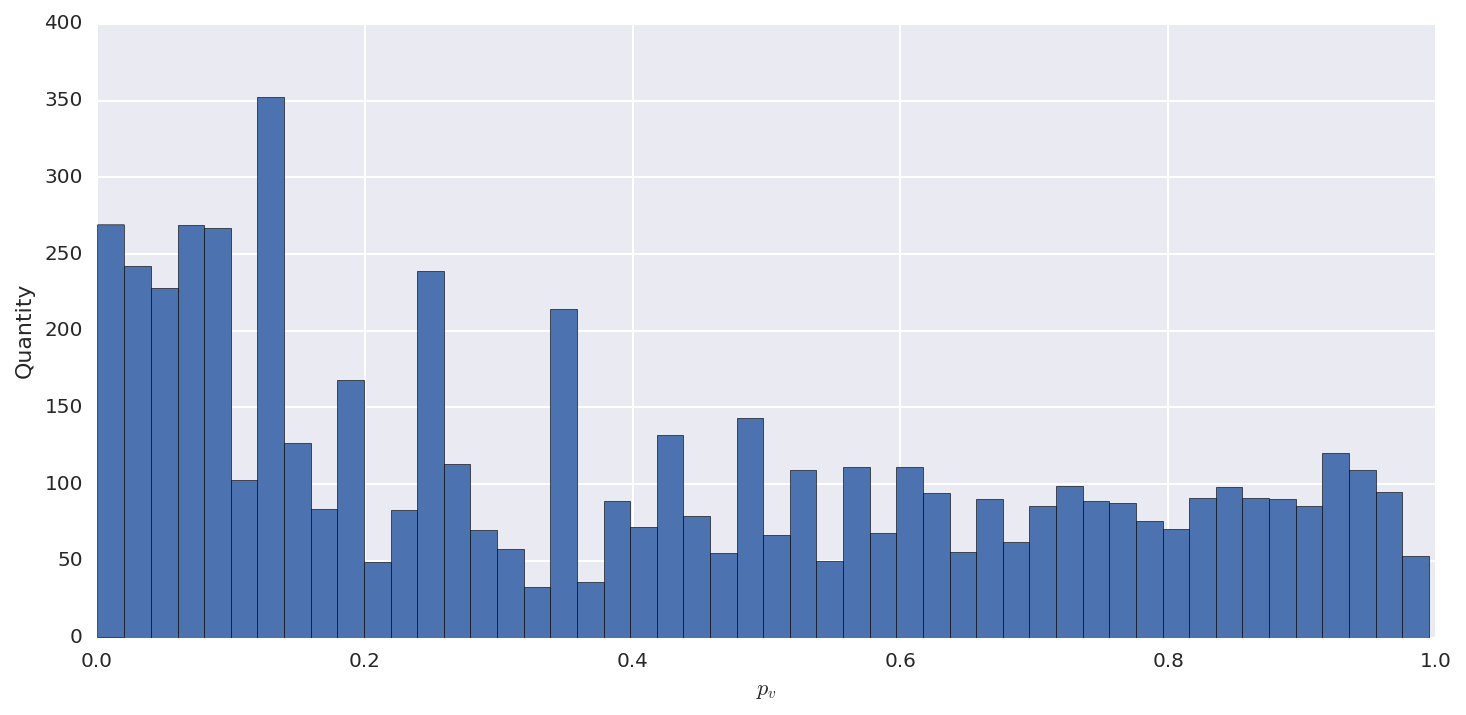
\includegraphics[height=.20\textheight]{figures/bayes/least1/hist_calls.png}
\end{subfigure}
\begin{subfigure}[b]{.49\textwidth}
	\raggedleft{}
	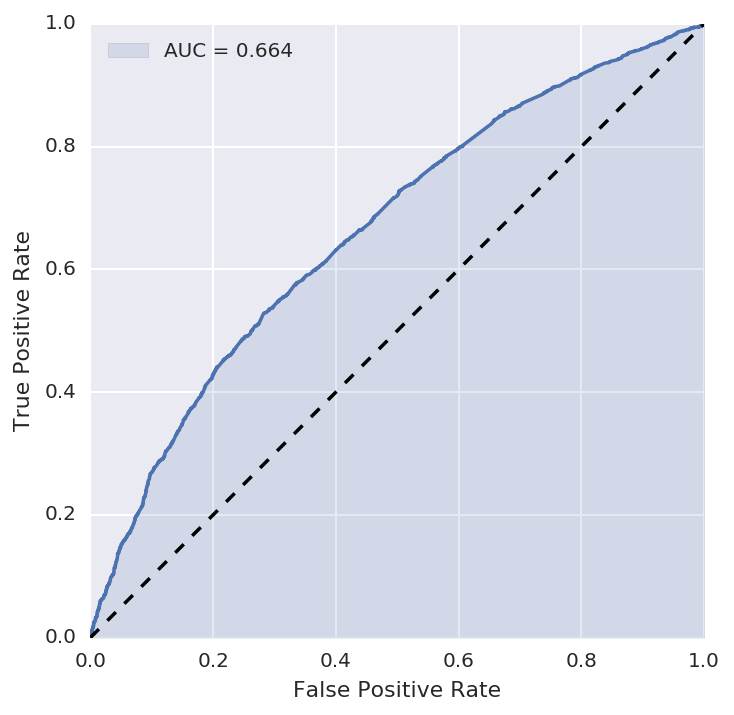
\includegraphics[height=.20\textheight]{figures/bayes/least1/roc_calls.png}
\end{subfigure}
\begin{subfigure}[b]{.49\textwidth}
	\raggedright{}
	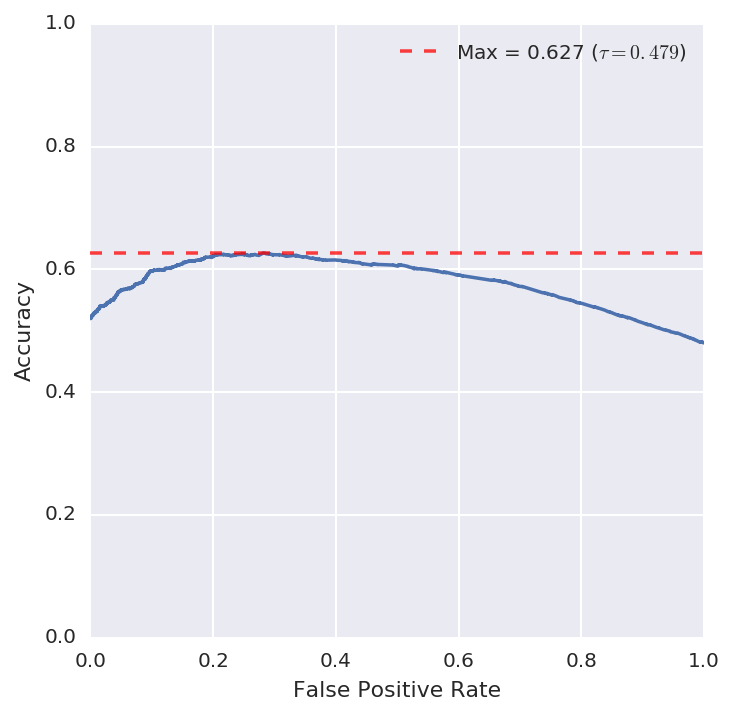
\includegraphics[height=.20\textheight]{figures/bayes/least1/accuracy_calls.png}
\end{subfigure}
\caption{Results for $\varpi = \calls$ when using $\hat{\Upsilon}^{\calls}$ instead of the whole set.}
\end{figure}

\begin{figure}[p]
\centering
\begin{subfigure}[t]{\textwidth}
	\centering
	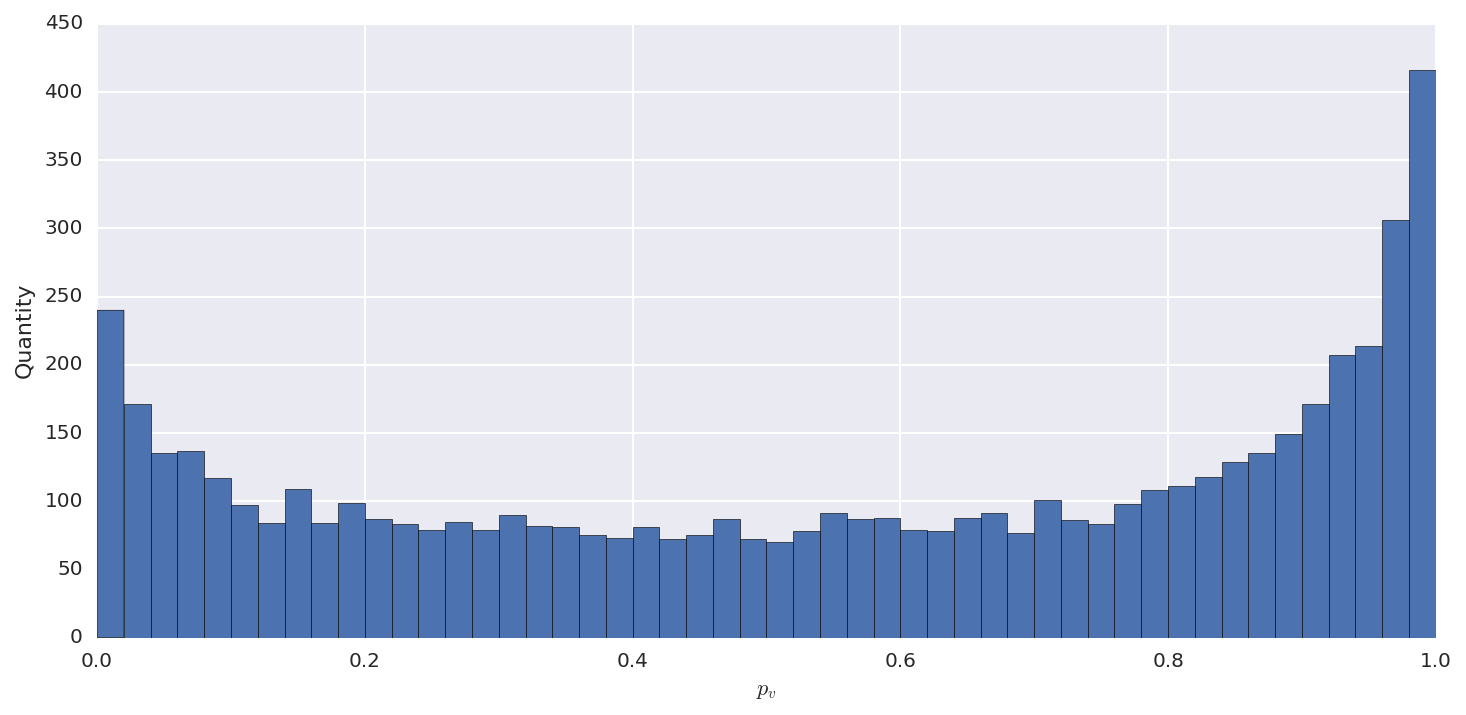
\includegraphics[height=.20\textheight]{figures/bayes/least1/hist_time.png}
\end{subfigure}
\begin{subfigure}[b]{.49\textwidth}
	\raggedleft{}
	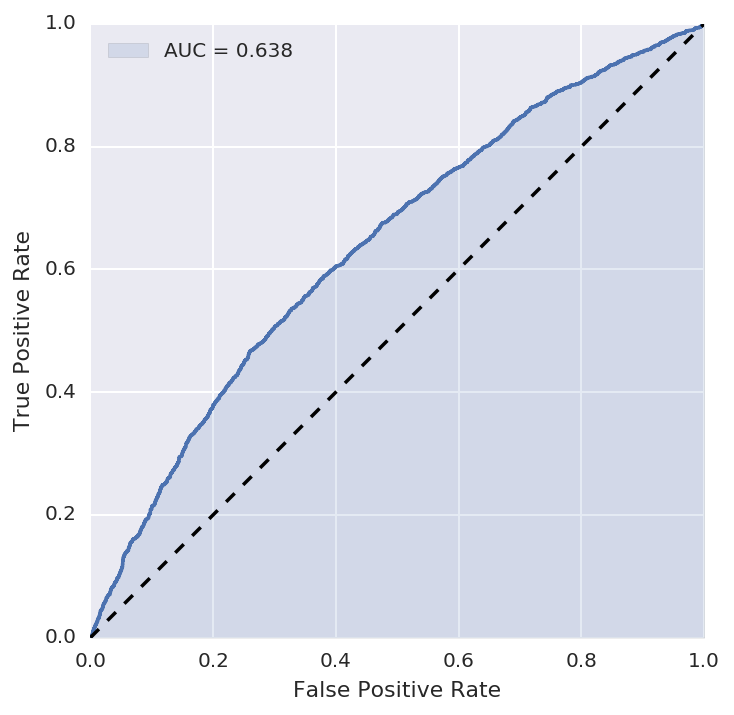
\includegraphics[height=.20\textheight]{figures/bayes/least1/roc_time.png}
\end{subfigure}
\begin{subfigure}[b]{.49\textwidth}
	\raggedright{}
	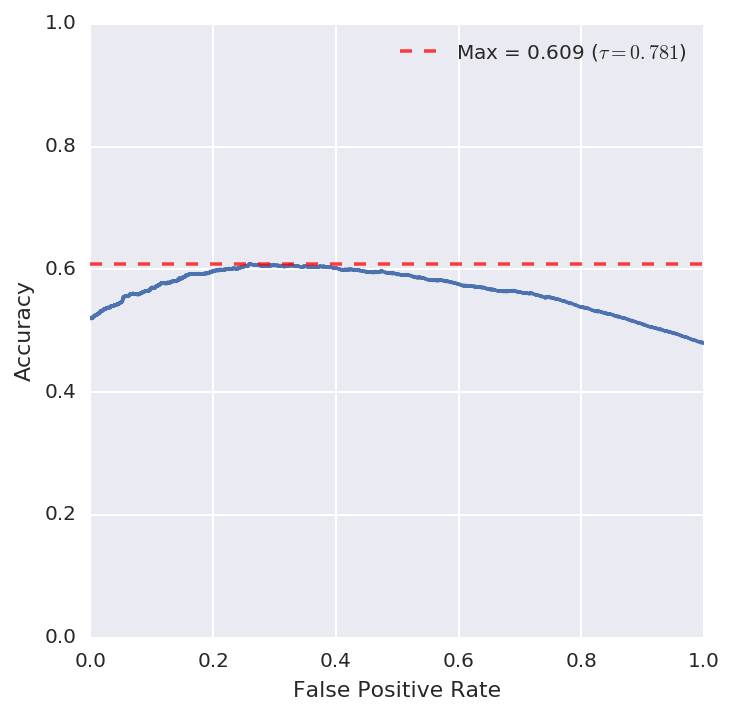
\includegraphics[height=.20\textheight]{figures/bayes/least1/accuracy_time.png}
\end{subfigure}
\caption{Results for $\varpi = \etime$ when using $\hat{\Upsilon}^{\calls}$ instead of the whole set. While the histogram is a lot more equitative than the one in Section~\ref{subsec:time_infer}, there are still the peaks at both ends are still distinguishable.}
\label{fig:time_infer_positive}
\end{figure}

\begin{figure}[p]
\centering
\begin{subfigure}[t]{\textwidth}
	\centering
	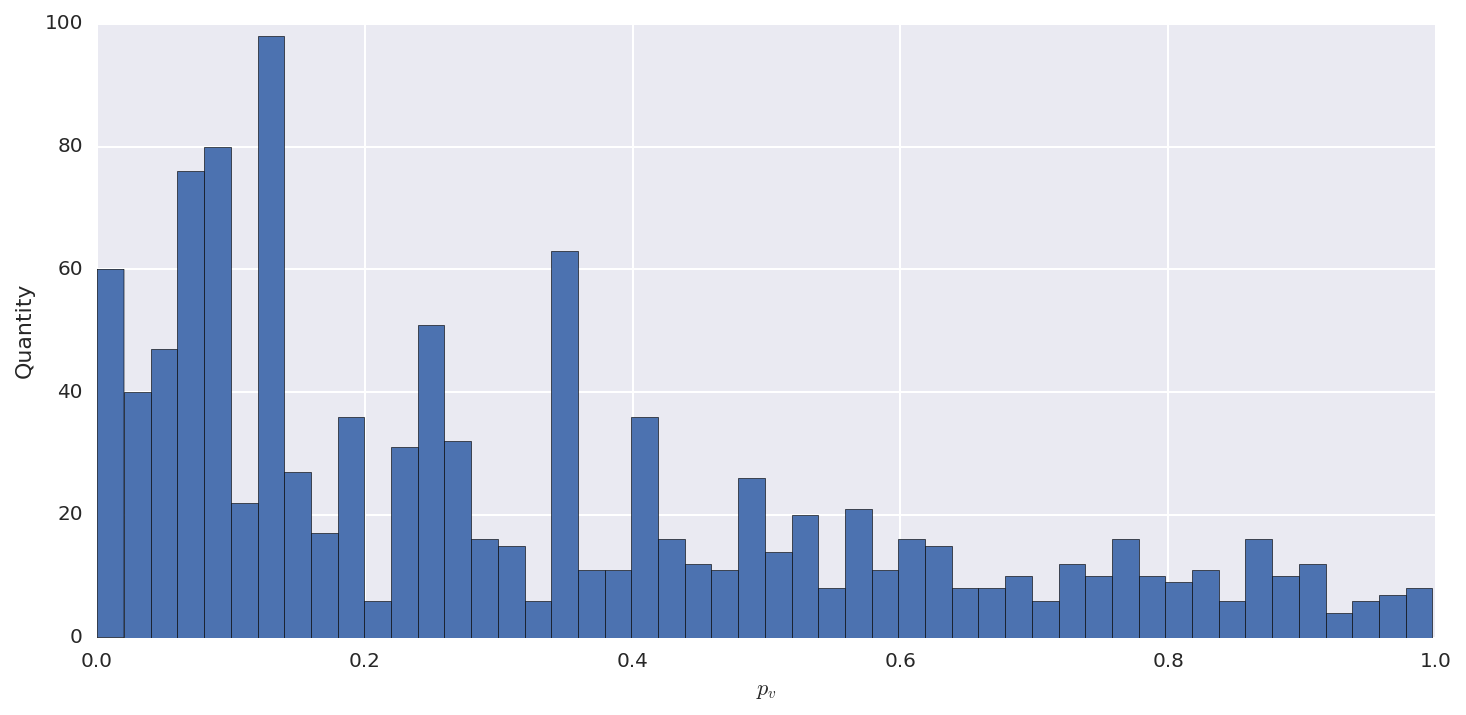
\includegraphics[height=.20\textheight]{figures/bayes/least1/hist_sms.png}
\end{subfigure}
\begin{subfigure}[b]{.49\textwidth}
	\raggedleft{}
	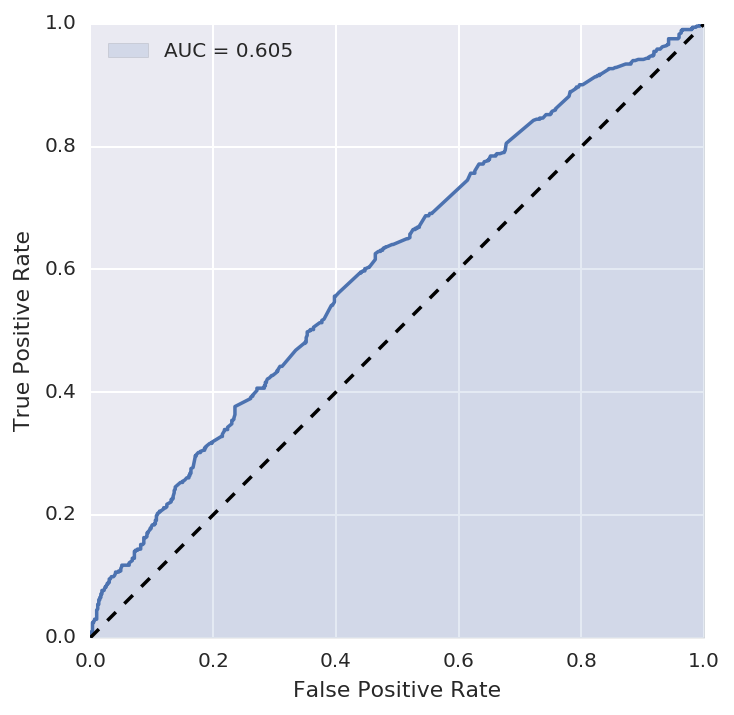
\includegraphics[height=.20\textheight]{figures/bayes/least1/roc_sms.png}
\end{subfigure}
\begin{subfigure}[b]{.49\textwidth}
	\raggedright{}
	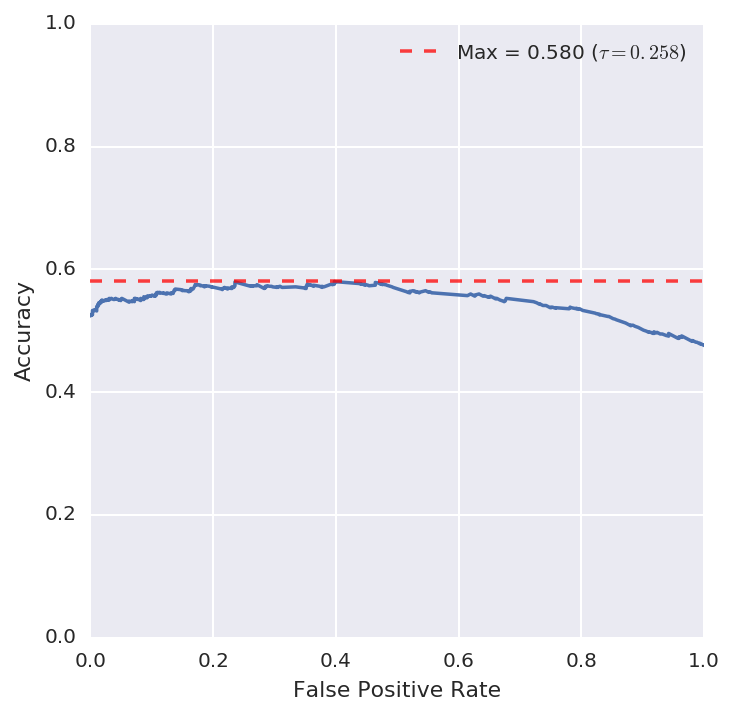
\includegraphics[height=.20\textheight]{figures/bayes/least1/accuracy_sms.png}
\end{subfigure}
\caption{Results for $\varpi = \sms$ when using $\hat{\Upsilon}^{\sms}$ instead of the whole set. As in the previous set, removing all cases where $\alpha = 1 \lor \beta = 1$ results in a more equitative histogram.}
\end{figure}

\begin{figure}[p]
\centering
\begin{subfigure}[t]{\textwidth}
	\centering
	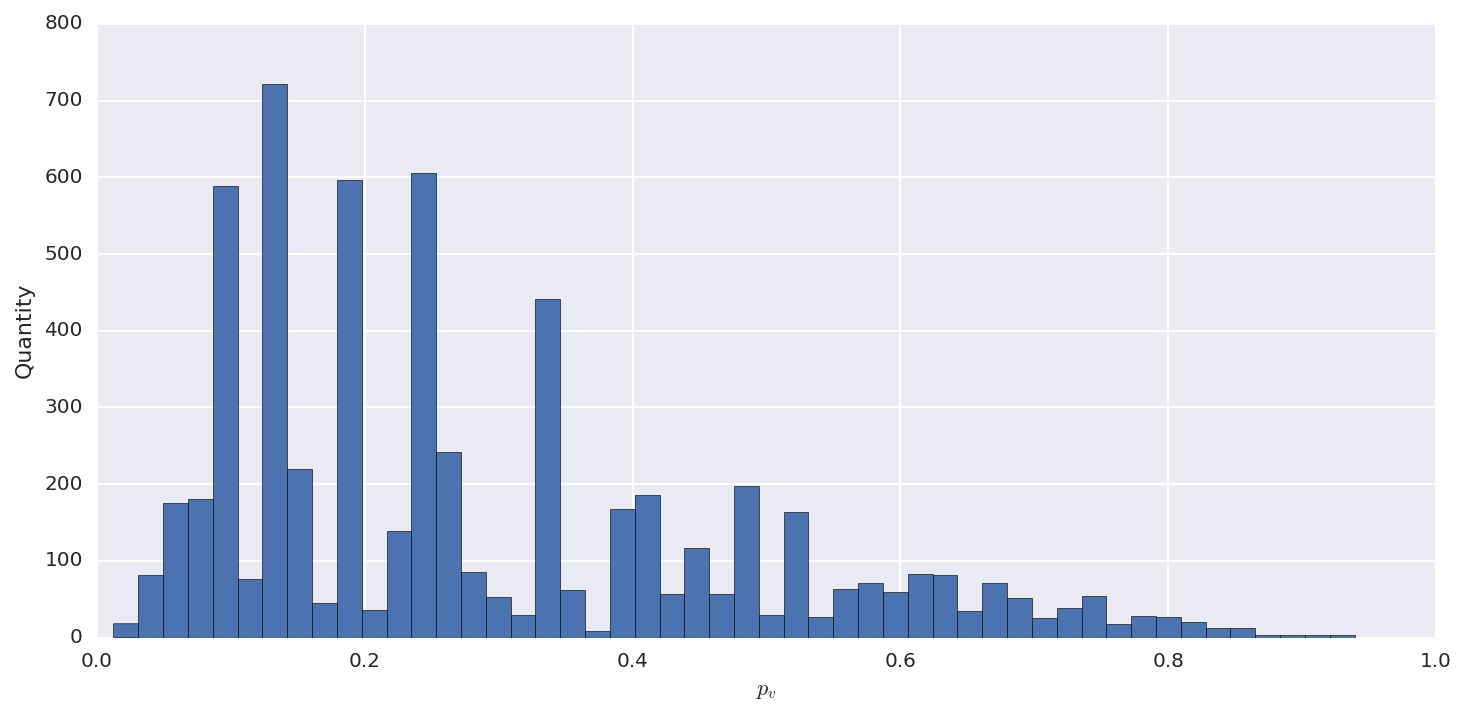
\includegraphics[height=.20\textheight]{figures/bayes/least1/hist_contacts.png}
\end{subfigure}
\begin{subfigure}[b]{.49\textwidth}
	\raggedleft{}
	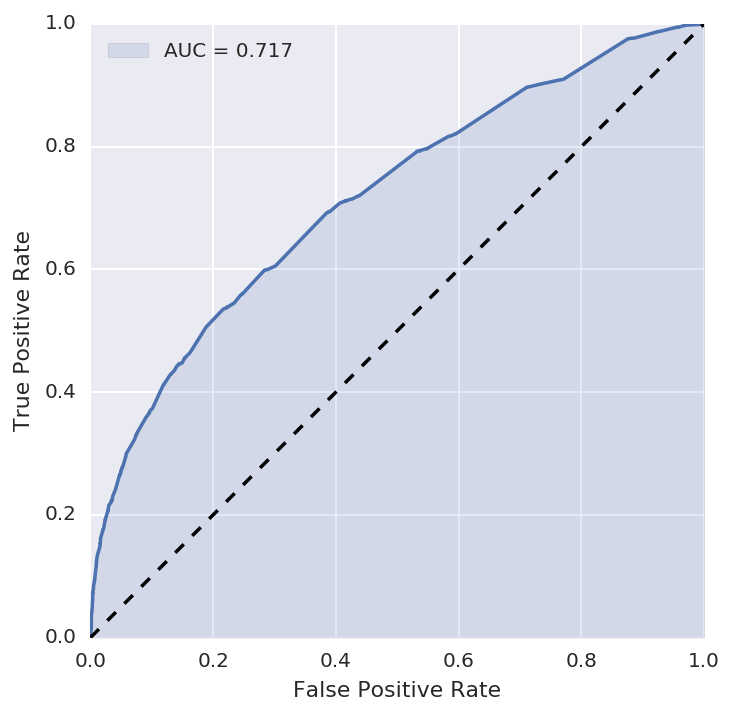
\includegraphics[height=.20\textheight]{figures/bayes/least1/roc_contacts.png}
\end{subfigure}
\begin{subfigure}[b]{.49\textwidth}
	\raggedright{}
	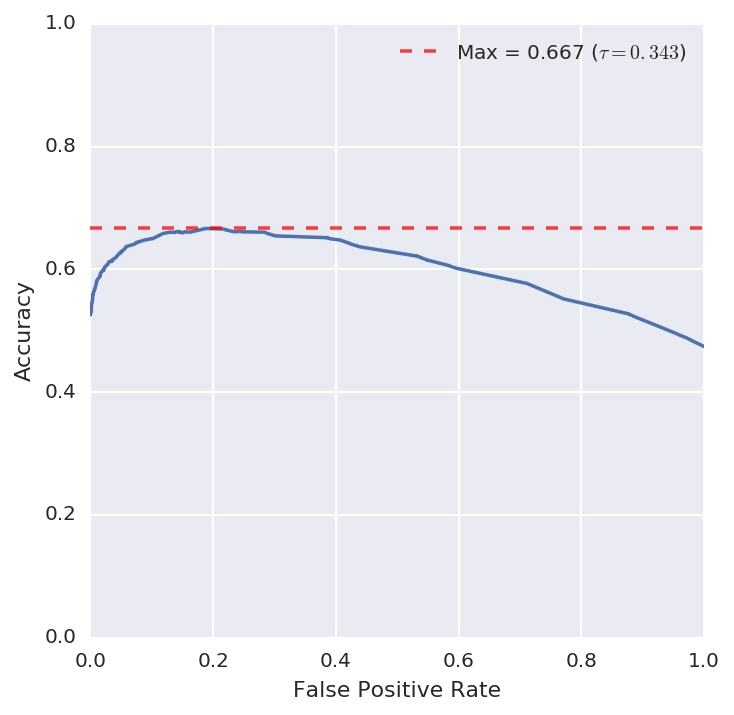
\includegraphics[height=.20\textheight]{figures/bayes/least1/accuracy_contacts.png}
\end{subfigure}
\caption{Results for $\varpi = \contacts$ when using $\hat{\Upsilon}$ instead of the whole set. Peaks are still visible due to the fact that it's easier to cluster users with the \emph{Socioeconomic Index} of their contacts.}
\end{figure}
